\subsection{Regular classes}
\label{subsec:library_of_transformations:type_level_transformations:regular_classes}

\begin{figure}
    \centering
    \begin{subfigure}{0.45\textwidth}
        \centering
        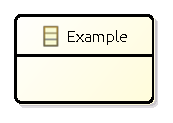
\includegraphics{images/05_library_of_transformations/02_type_level_transformations/01_regular_classes/class_type.pdf}
        \caption{$Tm_{Class}$ with $name = .\type{Example}$}
        \label{fig:library_of_transformations:type_level_transformations:regular_classes:visualisation:ecore}
    \end{subfigure}
    \begin{subfigure}{0.45\textwidth}
        \centering
        % To use this figure in your LaTeX document
% import the package groove/resources/groove2tikz.sty
%
\begin{tikzpicture}[scale=\tikzscale,name prefix=test-]
\node[type_node] (n0) at (0.950, -0.850) {\ml{\textbf{Example}}};

\end{tikzpicture}

        \caption{$TG_{Class}$ with $name = .\type{Example}$}
        \label{fig:library_of_transformations:type_level_transformations:regular_classes:visualisation:groove}
    \end{subfigure}
    \caption{Visualisation of the transformation of regular classes}
    \label{fig:library_of_transformations:type_level_transformations:regular_classes:visualisation}
\end{figure}

The first transformation that will be defined is a transformation of regular classes. A class without any additional properties is considered a regular class. The Ecore model for defining a regular class is given in the following definition:

\begin{defin}[Type model $Tm_{Class}$]
\label{defin:library_of_transformations:type_level_transformations:regular_classes:tmod_class}
Let $Tm_{Class}$ be the type model containing a regular class with identifier $name$. $Tm_{Class}$ is defined as:
\begin{align*}
Class =\ &\{name\} \\
Enum =\ &\{\} \\
UserDataType =\ &\{\} \\
Field =\ &\{\} \\
\mathrm{FieldSig} =\ &\{\} \\
EnumValue =\ &\{\} \\
Inh =\ &\{\} \\
Prop =\ &\{\} \\
Constant =\ &\{\} \\
\mathrm{ConstType} =\ &\{\}
\end{align*}
\isabellelref{tmod_class}{Ecore-GROOVE-Mapping-Library.ClassType}
\end{defin}

\begin{thm}[Correctness of $Tm_{Class}$]
\label{defin:library_of_transformations:type_level_transformations:regular_classes:tmod_class_correct}
$Tm_{Class}$ (\cref{defin:library_of_transformations:type_level_transformations:regular_classes:tmod_class}) is a consistent type model in the sense of \cref{defin:formalisations:ecore_formalisation:type_models:type_model_consistency}.
\isabellelref{tmod_class_correct}{Ecore-GROOVE-Mapping-Library.ClassType}
\end{thm}

A visual representation of $Tm_{Class}$ with identifier $.\type{Example}$ can be seen in \cref{fig:library_of_transformations:type_level_transformations:regular_classes:visualisation:ecore}. The correctness proof of $Tm_{Class}$ is trivial, and therefore not included here. The proof can be found as part of the Isabelle validated proofs.

In order to make composing transformation functions possible, $Tm_{Class}$ should be compatible with the type model it is combined with.

\begin{thm}[Correctness of $\mathrm{combine}(Tm, Tm_{Class})$]
\label{defin:library_of_transformations:type_level_transformations:regular_classes:tmod_class_combine_correct}
Assume a type model $Tm$ that is consistent in the sense of \cref{defin:formalisations:ecore_formalisation:type_models:type_model_consistency}. Then $Tm$ is compatible with $Tm_{Class}$ (in the sense of \cref{defin:transformation_framework:type_models_and_type_graphs:combining_type_models:compatibility}) if:
\begin{itemize}
    \item The identifier of the class in $Tm_{Class}$ is not yet an identifier for a class, enumeration type or user-defined data type in $Tm$;
    \item The identifier of the class in $Tm_{Class}$ is not in the namespace of any class, enumeration type or user-defined data type in $Tm$;
    \item None of the identifiers in any class, enumeration type or user-defined data type in $Tm$ is in the namespace of the class in $Tm_{Class}$.
\end{itemize}
\isabellelref{tmod_class_combine_correct}{Ecore-GROOVE-Mapping-Library.ClassType}
\end{thm}

\begin{proof}
Use \cref{defin:transformation_framework:type_models_and_type_graphs:combining_type_models:tmod_combine_merge_correct}. It is possible to show that all assumptions hold. Now we have shown that $\mathrm{combine}(Tm, Tm_{Class})$ is consistent in the sense of \cref{defin:formalisations:ecore_formalisation:type_models:type_model_consistency}.
\end{proof}

The definitions and theorems for a regular class within Ecore are now complete. 

\subsubsection{Encoding as node type}

A possible encoding for regular classes in Ecore is using a node type in GROOVE. This node type will get a transformed identifier as name. The encoding corresponding to $Tm_{Class}$ can then be represented as $TG_{Class}$, defined in the following definition:

\begin{defin}[Type graph $TG_{Class}$]
\label{defin:library_of_transformations:type_level_transformations:regular_classes:tg_class_as_node_type}
Let $TG_{Class}$ be the type graph containing a single node type which encodes a regular class $name$. $TG_{Class}$ is defined as:
\begin{align*}
NT =\ &\{\mathrm{ns\_\!to\_\!list}(name)\} \\
ET =\ &\{\} \\
\!\!\sqsubseteq\ =\ &\{( \mathrm{ns\_\!to\_\!list}(name), \mathrm{ns\_\!to\_\!list}(name) )\} \\
abs =\ &\{\} \\
\mathrm{mult} =\ &\{\} \\
contains =\ &\{\}
\end{align*}
\isabellelref{tg_class_as_node_type}{Ecore-GROOVE-Mapping-Library.ClassType}
\end{defin}

\begin{thm}[Correctness of $TG_{Class}$]
\label{defin:library_of_transformations:type_level_transformations:regular_classes:tg_class_as_node_type_correct}
$TG_{Class}$ (\cref{defin:library_of_transformations:type_level_transformations:regular_classes:tg_class_as_node_type}) is a valid type graph in the sense of \cref{defin:formalisations:groove_formalisation:type_graphs:type_graph_validity}.
\isabellelref{tg_class_as_node_type_correct}{Ecore-GROOVE-Mapping-Library.ClassType}
\end{thm}

A visual representation of $TG_{Class}$ with identifier $.\type{Example}$ can be seen in \cref{fig:library_of_transformations:type_level_transformations:regular_classes:visualisation:groove}. The correctness proof of $TG_{Class}$ is trivial, and therefore not included here. The proof can be found as part of the Isabelle validated proofs.

In order to make composing transformation functions possible, $TG_{Class}$ should be compatible with the type graph it is combined with.

\begin{thm}[Correctness of $\mathrm{combine}(TG, TG_{Class})$]
\label{defin:library_of_transformations:type_level_transformations:regular_classes:tg_class_as_node_type_combine_correct}
Assume a type graph $TG$ that is valid in the sense of \cref{defin:formalisations:groove_formalisation:type_graphs:type_graph_validity}. Then $TG$ is compatible with $TG_{Class}$ (in the sense of \cref{defin:transformation_framework:type_models_and_type_graphs:combining_type_graphs:compatibility}) if:
\begin{itemize}
    \item The node type of the encoded class in $TG_{Class}$ is not a node type in $TG$.
\end{itemize}
\isabellelref{tg_class_as_node_type_combine_correct}{Ecore-GROOVE-Mapping-Library.ClassType}
\end{thm}

\begin{proof}
Use \cref{defin:transformation_framework:type_models_and_type_graphs:combining_type_graphs:tg_combine_merge_correct}. It is possible to show that all assumptions hold. Now we have shown that $\mathrm{combine}(TG, TG_{Class})$ is valid in the sense of \cref{defin:formalisations:groove_formalisation:type_graphs:type_graph_validity}.
\end{proof}

The next definitions define the transformation function from $Tm_{Class}$ to $TG_{Class}$:

\begin{defin}[Transformation function $f_{Class}$]
\label{defin:library_of_transformations:type_level_transformations:regular_classes:tmod_class_to_tg_class_as_node_type}
The transformation function $f_{Class}(Tm)$ is defined as:
\begin{align*}
NT =\ &\{\mathrm{ns\_\!to\_\!list}(c) \mid c \in Class_{Tm}\} \\
ET =\ &\{\} \\
\!\!\sqsubseteq\ =\ &\{( \mathrm{ns\_\!to\_\!list}(c_1), \mathrm{ns\_\!to\_\!list}(c_2) ) \mid c_1 \in Class_{Tm} \land c_2 \in Class_{Tm} \} \\
abs =\ &\{\} \\
\mathrm{mult} =\ &\{\} \\
contains =\ &\{\}
\end{align*}
\isabellelref{tmod_class_to_tg_class_as_node_type}{Ecore-GROOVE-Mapping-Library.ClassType}
\end{defin}

\begin{thm}[Correctness of $f_{Class}$]
\label{defin:library_of_transformations:type_level_transformations:regular_classes:tmod_class_to_tg_class_as_node_type_func}
$f_{Class}(Tm)$ (\cref{defin:library_of_transformations:type_level_transformations:regular_classes:tmod_class_to_tg_class_as_node_type}) is a valid transformation function in the sense of \cref{defin:transformation_framework:type_models_and_type_graphs:combining_transformation_functions:transformation_function_type_model_type_graph} transforming $Tm_{Class}$ into $TG_{Class}$.
\isabellelref{tmod_class_to_tg_class_as_node_type_func}{Ecore-GROOVE-Mapping-Library.ClassType}
\end{thm}

The proof of the correctness of $f_{Class}$ will not be included here. Instead, it can be found in the validated Isabelle theories.

Finally, to complete the transformation, the transformation function that transforms $TG_{Class}$ into $Tm_{Class}$ is defined:

\begin{defin}[Transformation function $f'_{Class}$]
\label{defin:library_of_transformations:type_level_transformations:regular_classes:tg_class_as_node_type_to_tmod_class}
The transformation function $f'_{Class}(TG)$ is defined as:
\begin{align*}
Class =\ &\{\mathrm{list\_\!to\_\!ns}(n) \mid n \in NT_{TG}\} \\
Enum =\ &\{\} \\
UserDataType =\ &\{\} \\
Field =\ &\{\} \\
\mathrm{FieldSig} =\ &\{\} \\
EnumValue =\ &\{\} \\
Inh =\ &\{\} \\
Prop =\ &\{\} \\
Constant =\ &\{\} \\
\mathrm{ConstType} =\ &\{\}
\end{align*}
\isabellelref{tg_class_as_node_type_to_tmod_class}{Ecore-GROOVE-Mapping-Library.ClassType}
\end{defin}

\begin{thm}[Correctness of $f'_{Class}$]
\label{defin:library_of_transformations:type_level_transformations:regular_classes:tg_class_as_node_type_to_tmod_class_func}
$f'_{Class}(TG)$ (\cref{defin:library_of_transformations:type_level_transformations:regular_classes:tg_class_as_node_type_to_tmod_class}) is a valid transformation function in the sense of \cref{defin:transformation_framework:type_models_and_type_graphs:combining_transformation_functions:transformation_function_type_graph_type_model} transforming $TG_{Class}$ into $Tm_{Class}$.
\isabellelref{tg_class_as_node_type_to_tmod_class_func}{Ecore-GROOVE-Mapping-Library.ClassType}
\end{thm}

Once more, the correctness proof is not included here but can be found in the validated Isabelle proofs of this thesis.